\documentclass{article}

\usepackage[margin=0.5in]{geometry}
\usepackage{multicol}
\usepackage{tikz}

\title{Triangles Set B}
\date{}
\author{}

\begin{document}
\maketitle
\noindent Problems should be solved without calculators unless otherwise specified.
Remember to explain how you solved a problem.
\begin{multicols}{2}
    \begin{enumerate}
        \item An ant is crawling along the outside of the box.
            What is the shortest distance he can walk from $A$ to $B$ along the path shown?
            \begin{center}
                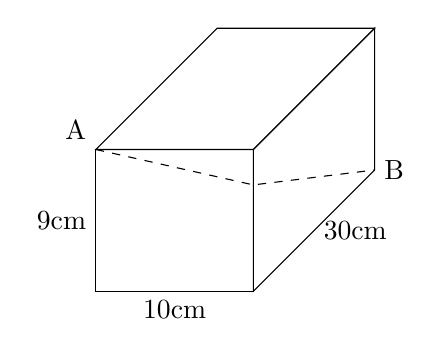
\begin{tikzpicture}
                    \coordinate[label=above left:A] (A) at (0,1.8,4);
                    \coordinate[label=right:B] (B) at (2,0,0);
                    \draw (0,0,4) -- node[left] {9cm} (0,1.8,4) -- (A) -- (2,1.8,4) -- (2,0,4) -- node[below] {10cm} (0,0,4) -- cycle;
                    \draw (B) -- node[right] {30cm} (2,0,4) -- (2,0,4) -- (2,1.8,4) -- (2,1.8,0) -- cycle;
                    \draw (0,1.8,0) -- (2,1.8,0) -- (2, 1.8, 4) -- (A) -- cycle;
                    \draw[dashed] (A) -- (2,1.35,4) -- (B);
                \end{tikzpicture}
            \end{center}
            \vspace{3cm}
        \item There is a shorter path from $A$ to $B$ in the diagram above.
            What is the shortest distance along the outside of the box from $A$ to $B$?
            Express your answer as a decimal rounded to the nearest tenth.
            \vspace{3cm}
        \item An equilateral triangle is stacked above a square as shown, with a circle inscribed inside the square and two stacked circles inscribed in the triangles so that they are tangent to each other.
            What is the ratio of the area of the smallest circle to the area of the largest circle?
            Express your answer as a common fraction.
            \begin{center}
                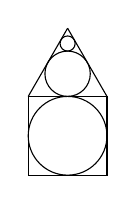
\begin{tikzpicture}
                    \draw (0,0) -- (1,0) -- (1,1) -- (0,1) -- cycle;
                    \draw (0.5,0.5) circle (0.5cm);
                    \draw (0,1) -- ++(60:1);
                    \draw (1,1) -- ++(120:1);
                    \draw (0.5, 1.288) circle (0.288);
                    \draw (0.5, 1.672) circle (0.096);
                \end{tikzpicture}
            \end{center}
            \vspace{3cm}
        \item What is the height of a STOP sign (regular octagon) whose sides are one foot long?
            \vspace{3cm}
        \item Three circles, each having a radius of $4$ units, are externally tangent to each other.
            A triangle joins the centers of the circles.
            What is the area of the shaded region within the triangle but outside the circles?
            Express your answer as a decimal to the nearest tenth.
            \begin{center}
                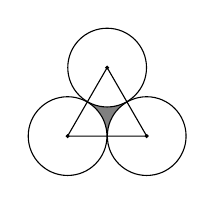
\begin{tikzpicture}
                    \draw[fill=gray] (90:0.58) -- (210:0.58) -- (330:0.58) -- cycle;
                    \foreach \angle in {90, 210, 330}
                    {
                        \begin{scope}
                            \clip (\angle:0.58) circle (0.5cm);
                            \fill[white] (\angle:0.58) circle (0.5cm);
                        \end{scope}
                        \draw (\angle:0.58) circle (0.5cm);
                        \filldraw (\angle:0.58) circle (0.5pt);
                    }
                    \draw (90:0.58) -- (210:0.58) -- (330:0.58) -- cycle;
                \end{tikzpicture}
            \end{center}
            \vspace{3cm}
    \end{enumerate}
\end{multicols}
\end{document}